\documentclass{standalone}
\usepackage[usenames, dvipsnames]{xcolor}
\usepackage{amsmath, tikz, pgfplots}
\usetikzlibrary{arrows.meta}
\usepgfplotslibrary{fillbetween}

\pgfmathsetmacro{\smi}{0.075}

\begin{document}
	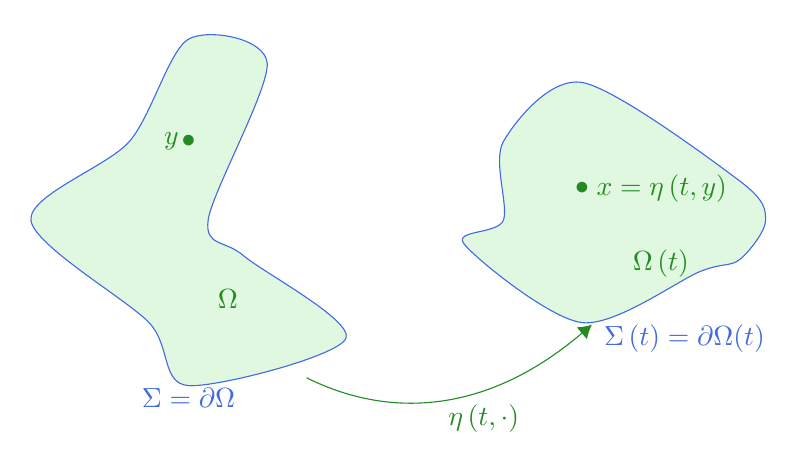
\begin{tikzpicture}
		% The reference set Omega_0 [part 1, to ensure appropriate layering with the diagram of the microstructure]
		\draw [RoyalBlue, fill=LimeGreen, fill opacity=0.15] plot [smooth cycle] coordinates {(-3, 2.3) (-2, 2) (-2.75, 0) (-2.3, -0.45) (-1, -1.5) (-3, -2.1) (-3.5, -1.3) (-5, 0) (-3.75, 1)};
		% The reference configuration of the microstructure at y
% % 		\draw [Thistle] (-3, 1) -- (-2.49, 3.1);
% 		\draw [Thistle] (-3, 1) -- (-1.6, 2.7);
% 		\draw [Thistle, fill=White] (-2, 3) circle [radius = 0.5];
% 		\draw [Thistle, ->] (-2, 3) -- (-2, 3.4);
% 		\draw [Thistle, ->] (-2, 3) -- (-1.6, 3);
% 		\draw [Thistle, ->] (-2, 3) -- (-2.225, 2.775);
		% The reference micro-inertia tensor
% 		\node[left, RoyalBlue] at (-2.5, 3) {$\mathcal{I}_0$};
% 		\draw [fill=White] plot [smooth cycle] coordinates {
% 			(-2+\smi*1.5, 3+\smi*0)
% 			(-2+\smi*2, 3+\smi*-1)
% 			(-2+\smi*3, 3+\smi*-1.5)
% 			(-2+\smi*2, 3+\smi*-2.5)
% 			(-2+\smi*0, 3+\smi*-3)
% 			(-2+\smi*-1, 3+\smi*-2)
% 			(-2+\smi*-1.5, 3+\smi*0)
% 			(-2+\smi*-2, 3+\smi*1)
% 			(-2+\smi*-1, 3+\smi*2.5)
% 			(-2+\smi*0.5, 3+\smi*3)
% 			(-2+\smi*1.5, 3+\smi*2)
% 		};
% 		\draw [RoyalBlue, fill=RoyalBlue, opacity=0.2] plot [smooth cycle] coordinates {
% 			(-2+\smi*1.5, 3+\smi*0)
% 			(-2+\smi*2, 3+\smi*-1)
% 			(-2+\smi*3, 3+\smi*-1.5)
% 			(-2+\smi*2, 3+\smi*-2.5)
% 			(-2+\smi*0, 3+\smi*-3)
% 			(-2+\smi*-1, 3+\smi*-2)
% 			(-2+\smi*-1.5, 3+\smi*0)
% 			(-2+\smi*-2, 3+\smi*1)
% 			(-2+\smi*-1, 3+\smi*2.5)
% 			(-2+\smi*0.5, 3+\smi*3)
% 			(-2+\smi*1.5, 3+\smi*2)
% 		};
		% The reference set Omega_0 [part 2]
		\node [ForestGreen] at (-2.5, -1) {$\Omega$};
 		\node [RoyalBlue] at (-3, -2.25) {$\Sigma = \partial \Omega$};
		% The reference set Omega_0 [part 2]
% 		\node [ForestGreen] at (-3, -2.5) {$\Omega_0$};
		\node [ForestGreen] at (-3, 1) {$\bullet$};
		\node [left, ForestGreen] at (-3, 1) {$y$};
		% The continuum at time t, i.e. the set Omega(t) [part 1]
		\draw [RoyalBlue, fill=LimeGreen, fill opacity=0.15] plot [smooth cycle] coordinates {(1, 0) (1, 1) (2, 1.75) (4, .5) (4.33, 0) (4, -.5) (3.5, -.65) (2, -1.3) (.5, -.3)};
		% The configuration of the microstructure at x at time t
% 		\draw [Thistle] (2, 0) -- (2.51, 2.1);
% 		\draw [Thistle] (2, 0) -- (3.4, 1.7);
% 		\draw [Thistle, fill=White] (3, 2) circle [radius = 0.5];
% 		\draw [Thistle, ->] (3, 2) -- (3, 2.4);
% 		\draw [Thistle, ->] (3, 2) -- (3.4, 2);
% 		\draw [Thistle, ->] (3, 2) -- (2.725, 1.725);
		% The micro-inertia tensor in the deformed micro-continuum
% 		\node[right, RoyalBlue] at (3.5, 2) {$\mathcal{I} (t,y) = Q \, \mathcal{I}_0 \, Q^T$};
% 		\draw [fill=White] plot [smooth cycle] coordinates {
% 			(3+\smi*0, 2-\smi*1.5)
% 			(3+\smi*-1, 2-\smi*2)
% 			(3+\smi*-1.5, 2-\smi*3)
% 			(3+\smi*-2.5, 2-\smi*2)
% 			(3+\smi*-3, 2-\smi*0)
% 			(3+\smi*-2, 2-\smi*-1)
% 			(3+\smi*0, 2-\smi*-1.5)
% 			(3+\smi*1, 2-\smi*-2)
% 			(3+\smi*2.5, 2-\smi*-1)
% 			(3+\smi*3, 2-\smi*0.5)
% 			(3+\smi*2, 2-\smi*1.5)
% 		};
% 		\draw [RoyalBlue, fill=RoyalBlue, fill opacity=0.2] plot [smooth cycle] coordinates {
% 			(3+\smi*0, 2-\smi*1.5)
% 			(3+\smi*-1, 2-\smi*2)
% 			(3+\smi*-1.5, 2-\smi*3)
% 			(3+\smi*-2.5, 2-\smi*2)
% 			(3+\smi*-3, 2-\smi*0)
% 			(3+\smi*-2, 2-\smi*-1)
% 			(3+\smi*0, 2-\smi*-1.5)
% 			(3+\smi*1, 2-\smi*-2)
% 			(3+\smi*2.5, 2-\smi*-1)
% 			(3+\smi*3, 2-\smi*0.5)
% 			(3+\smi*2, 2-\smi*1.5)
% 		};
		% The continuum at time t, i.e. the set Omega(t) [part 2]
		\node [ForestGreen] at (3, -.55) {$\Omega\,(t)$};
		\node [RoyalBlue] at (3.3, -1.5) {$\Sigma\,(t) = \partial \Omega (t)$};
		% The continuum at time t, i.e. the set Omega(t) [part 2]
% 		\node [ForestGreen] at (3, -1.5) {$\Omega\,(t)$};
		\node [ForestGreen] at (2, .4) {$\bullet$};
		\node [right, ForestGreen] at (2, .4) {$\,x = \eta\,(t,y)$};
		% Arrow depicting the macro-motion
		\draw [-{Latex[width=2mm]},  ForestGreen] (-1.5, -2) .. controls (-0.5, -2.5) and (0.75, -2.5) .. (2.125, -1.325);
		\node [ForestGreen] at (0.75, -2.525) {$\eta\,(t,\cdot)$};
		
		
	
		
		
		% Arrow depicting the micro-motion
% 		\draw [-{Latex[width=2mm]},  Thistle] (-1.1, 3.4) .. controls (0.5, 4) and (1.75, 3.25) .. (2.4, 2.6);
% 		\node [Thistle] at (1.4, 3.75) {$Q(t,y)$};
	\end{tikzpicture}	
\end{document}
